\section{Auswertung}
\label{sec:Auswertung}
Alle nachfolgenden Plots und Regressionen wurden mithilfe von python erstellt und berechnet.

\subsection{Entladevorgang}
Zuerst wird der Entladevorgang des Kondensators betrachtet. Das Oszilloskop zeigt Abbildung \ref{fig:oszi1}. Aus diesem Graphen werden einige
Werte abgelesen und in Tabelle \ref{tab:entlade} dargestellt. Das Nullniveau befindet sich bei
\begin{equation*}
  U_0 = \SI{17.6}{V} \,.
\end{equation*}

\begin{figure}[H]
  \centering
  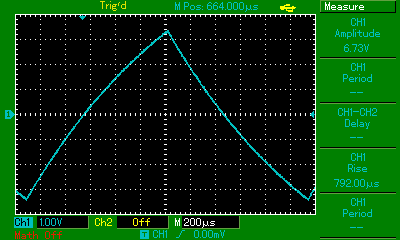
\includegraphics{bilder/MAP002.png}
  \caption{Lade- und Entladevorgang des Kondensators.}
  \label{fig:oszi1}
\end{figure}

\begin{table}
  \centering
  \caption{Entladevorgang des Kondensators.}
  \label{tab:entlade}
  \begin{tabular}{c | S S S S S S S S S S}
    $t$ in ms & 0.1 & 0.2 & 0.3 & 0.4 & 0.5 & 0.6 & 0.7 & 0.8 & 0.9 & 1.0 \\
    \hline
    $U_\text{C}$ in V & 6.0 & 5.2 & 4.5 & 3.8 & 3.1 & 2.6 & 2.0 & 1.5 & 1.0 & 0.6
  \end{tabular}
\end{table}

Diese Werte werden in Abbildung \ref{fig:entlade} zusammen mit der entsprechenden linearen Regression halblogarithmisch aufgetragen.

Die Regression berechnet sich nach
\begin{equation*}
  f(x) = ax
\end{equation*}
mit $f(x) = \log(\frac{U_\text{C}}{U_0})$ und $a = -\frac{1}{RC}$ und es ergibt sich der Wert
\begin{equation*}
  a = \SI{-3.335 \pm 0.180}{kHz} \,.
\end{equation*}
Daraus folgt
\begin{equation*}
  RC = -\frac{1}{a} = \SI{0.300 \pm 0.016}{ms} \,.
\end{equation*}
\begin{figure}[H]
  \centering
  \includegraphics{build/a.pdf}
  \caption{Kondensatorspannung beim Entladevorgang.}
  \label{fig:entlade}
\end{figure}

\subsection{Amplitude und Phasenverschiebung}
Als nächstes werden die Amplitude $U_\text{C}$ und die Phasenverschiebung $\phi$ abhängig von der Frequenz $\nu$ betrachtet und die
Messergebnisse in Tabelle \ref{tab:messwerte} aufgetragen. Dabei wird die Phasenverschiebung $\phi$ nach \eqref{eq:phi} berechnet.

\begin{table}[H]
  \centering
  \caption{Messwerte der Frequenzabhängigkeit der Amplitude und der Phasenverschiebung.}
  \label{tab:messwerte}
  \begin{tabular}{S[table-format=5] S[table-format=2.3] S[table-format=1.3] S[table-format=3.3] S[table-format=1.3]}
    {$\nu \:/\: \si{\hertz}$} & {$U_\text{C} \:/\: \si{V}$} & {$ a \:/\: \si{ms}$} & {$b \:/\: \si{ms}$} & {$\phi \:/\: \si{rad}$} \\
    \midrule
    10    & 21.380 & 0.000 & 100.000 & 0.000 \\
    50    & 19.800 & 1.600 & 20.000  & 0.503 \\
    100   & 15.440 & 1.400 & 10.000  & 0.880 \\
    200   & 10.300 & 0.880 & 5.000   & 1.106 \\
    300   & 7.130  & 0.640 & 3.330   & 1.208 \\
    400   & 5.540  & 0.520 & 2.500   & 1.307 \\
    500   & 4.440  & 0.440 & 2.000   & 1.382 \\
    1000  & 2.300  & 0.240 & 1.000   & 1.508 \\
    2000  & 1.130  & 0.128 & 0.500   & 1.608 \\
    3000  & 0.792  & 0.088 & 0.330   & 1.676 \\
    4000  & 0.594  & 0.068 & 0.250   & 1.709 \\
    5000  & 0.495  & 0.056 & 0.200   & 1.759 \\
    10000 & 0.238  & 0.026 & 0.100   & 1.634 \\
    20000 & 0.135  & 0.014 & 0.050   & 1.759 \\
    30000 & 0.095  & 0.010 & 0.033   & 1.904 \\
  \end{tabular}
\end{table}

Die Kondensatorspannung $U_\text{C}$ in Abhängigkeit der Frequenz ist in Abbildung \ref{fig:amplitude} dargestellt. Dabei ist $U_0 = \SI{21.6}{V}$.
\begin{figure}[H]
  \centering
  \includegraphics{build/b1.pdf}
  \caption{Frequenzabhängigkeit der Kondensatorspannung.}
  \label{fig:amplitude}
\end{figure}

Die nicht-lineare Regression wird nach
\begin{equation*}
  f(x) = \frac{1}{\sqrt{1+\left(\frac{\nu}{2\symup{\pi}}^2a^2\right)}}
\end{equation*}
mit $a = RC$ wie in \eqref{eq:tiefpass} berechnet und liefert den Wert
\begin{equation*}
  RC = \SI{0.0593 \pm 0.0005}{s} \,.
\end{equation*}
Es zeigt sich, dass das auf diese Weise ermittelte $RC$ deutlich größer ist, als das $RC$ aus der linearen Regression des Entladevorgangs.

Die Phasenverschiebung $\phi$ abhängig von der Frequenz ist mitsamt einer Regression der Form
\begin{equation*}
  \phi = \arctan(-\frac{\nu}{2\symup{\pi}}a) \,,
\end{equation*}
analog zu Gleichung \eqref{eq:phase}, in Abbildung \ref{fig:phasenversch} dargestellt.

\begin{figure}[H]
  \centering
  \includegraphics{build/b2.pdf}
  \caption{Frequenzabhängigkeit der Phasenverschiebung.}
  \label{fig:phasenversch}
\end{figure}

Die Regression liefert den Wert
\begin{equation*}
  a = RC = \SI{0.068 \pm 0.011}{s} \,,
\end{equation*}
welcher ähnlich zu dem Wert ist, welcher sich aus der Frequenzabhängigkeit der Kondensatorspannung ergab.

Der Zusammenhang zwischen der Spannungsamplitude $U_\text{C}$ und der Phasenverschiebung $\phi$ ist in Abbildung \ref{fig:eisbaer} in einem
Polarplot aufgetragen. Dabei sind sowohl die Theoriekurve (schwarz) als auch die Messwerte (rot) dargestellt.
\begin{figure}[H]
  \centering
  \includegraphics{build/b3.pdf}
  \caption{Abhängigkeit zwischen Spannungsamplitude und Phase.}
  \label{fig:eisbaer}
\end{figure}

\subsection{Integrator}
Gleichung \eqref{eq:integrator} zeigt, dass der RC-Kreis auch als Integrator verwendet werden kann.
In Abbildung \ref{fig:oszi2} ist das Oszilloskopbild der Integration einer Sinusspannung mit
\begin{align*}
  f(x) &= A\sin(x) \\
  F(x) &= -A\cos(x)
\end{align*}
zu sehen.
\begin{figure}[H]
  \centering
  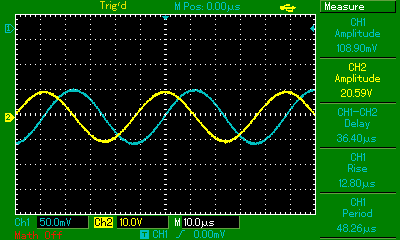
\includegraphics{bilder/MAP003.png}
  \caption{Integration einer Sinusspannung.}
  \label{fig:oszi2}
\end{figure}

Für eine Dreieckspannung gilt
\begin{align*}
  f(x) &= \begin{cases} &Ax \text{  für } 2\symup{\pi} n < x \leq 2\symup{\pi} n + 1 \\
                        &-Ax \text{  für } 2\symup{\pi} n + 1 < x \leq 2\symup{\pi} (n+1) \end{cases} \\
  F(x) &= \begin{cases} &\frac{1}{2} Ax^2 \text{  für } 2\symup{\pi} n < x \leq 2\symup{\pi} n + 1 \\
                        &-\frac{1}{2} Ax^2 \text{  für } 2\symup{\pi} n + 1 < x \leq 2\symup{\pi} (n+1) \end{cases}
\end{align*}
und das entsprechende Oszilloskopaufnahme ist in Abbildung \ref{fig:oszi3} dargestellt.
\begin{figure}[H]
  \centering
  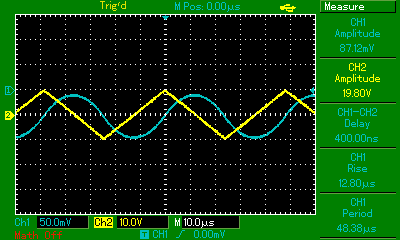
\includegraphics{bilder/MAP005.png}
  \caption{Integration einer Dreiecksspannung.}
  \label{fig:oszi3}
\end{figure}

Auch eine Rechteckspannung mit
\begin{align*}
  f(x) &= \begin{cases} &A \text{  für } 2\symup{\pi} n < x \leq 2\symup{\pi} n + 1 \\
                        &-A \text{  für } 2\symup{\pi} n + 1 < x \leq 2\symup{\pi} (n+1) \end{cases} \\
  F(x) &= \begin{cases} &Ax \text{  für } 2\symup{\pi} n < x \leq 2\symup{\pi} n + 1 \\
                        &-Ax \text{  für } 2\symup{\pi} n + 1 < x \leq 2\symup{\pi} (n+1) \end{cases}
\end{align*}
lässt sich im RC-Kreis integrieren, wie Abbildung \ref{fig:oszi4} zeigt.
\begin{figure}[H]
  \centering
  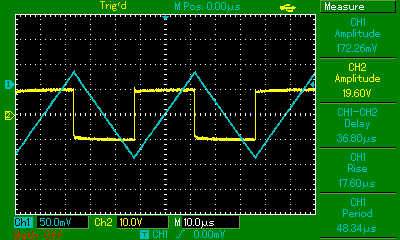
\includegraphics{bilder/MAP006.png}
  \caption{Integration einer Rechteckspannung.}
  \label{fig:oszi4}
\end{figure}

In den Aufnahmen des Oszilloskops sind die Eingangsspannungen jeweils in gelb, die Ausgangsspannungen in blau dargestellt.\newpage
